\documentclass[eng, pl, oneside, openright, final, openbib]{mgr}\DeclareUnicodeCharacter{0301}{\'{e}}
\usepackage{polski}
\usepackage[utf8]{inputenc}
\usepackage{comment}
\usepackage{babel}
\usepackage{amsmath}
\usepackage{amsfonts}
\usepackage{listings}
\newtheorem{twr}{Twierdzenie}
\def\listtablename{Spis tabel}
\def\tablename{Tabela. }
\usepackage{tikz}
\usepackage{array}
\usepackage{algorithmicx}
\usepackage{makeidx}
\usetikzlibrary{shapes.geometric, arrows}
\author{}
\title{Projektowanie cyfrowych filtrow z wykorzystaniem metod inteligentnych systemów przetwarzania sygnałów na przykładzie algorytmów ewolucyjnych}
\engtitle{The design approaches of digital filters based on evolutionary optimization techniques}
\supervisor{}
\field{Telekomunikacja (TEL)}
\specialisation{Multimedia w telekomunikacji (TMU)}
\date{2022}

\begin{document}
\maketitle

\pagenumbering{arabic}

\begin{figure}[b]
Oświadczam, świadomy(-a) odpowiedzialności karnej za poświadczenie
nieprawdy, że niniejszy projekt inżynierski wykonałem(-am) osobiście i że nie
korzystałem(-am) ze źródeł innych niż wymienione w pracy.
\newline
Wrocław, dnia ……………. Podpis dyplomanta ………………………….
\end{figure}

\tableofcontents


\chapter{Wstęp}
\section{Cel pracy dyplomowej}
Celem pracy dyplomowej jest skonstruowanie oraz przebadanie algorytmów bazujących na strategiach ewolucyjnych dla problemu projektowania filtrów cyfrowych (Finity Impulse Response) o wielu pasmach zaporowych oraz liniowej fazie w pasmach przepustowych przy ograniczeniu na wysokości zafalowań w obu pasmach.  
  
\section{Założenia pracy dyplomowej}
Założeniem projektu inżynierskiego jest skorzystanie z dostępnych narzędzi wymienionych w rozdziale pt. "Wykorzystane narzędzia". Następnie znalezienie dostępnych materiałów na temat implementacji algorytmów ewolucyjnych oraz filtrów cyfrowych. Kolejnym elementem pracy dyplomowej będzie przeanalizowanie dostępnych materiałów i na ich podstawie implementacja tytułowych algorytmów. W zamyślę autora pracy będzie implementacja dwóch lub więcej takich algorytmów z wykorzystaniem metod  strategii ewolucyjnych. Po zakończeniu fazy implementacji należy zweryfikować czy rozwiązania są prawidłowowo zrealizowane oraz w razie negatywnego wyniku, wprowadzenie poprawek. Kolejnym etapem będzie sprawdzenie szybkości wykonywania badanych algorytmów. Ostatecznym etapem wieńczącym pracę będzie zredagowanie podsumowania z odpowiedzią na pytanie, czy tytułowe algorytmy są w stanie zaprojektować filtr w sposób optymalny.
 
\section*{Streszczenie w języku angielsku}
The main target of the thesis is to verify how evolutionary algorithms will cope with the problem of designing and producing a digital filter with a finite impulse response. The problem will be solved for the general case, but for the thesis considerations, the implementation will be supported by an example of a digital filter of n = 99 order. This means that the filter will consist of 240 samples. The next necessary step after creating the filter will be the necessity to verify the results in terms of correctness and effectiveness against the background of other algorithms that will be presented in this paper. The next step will include checking the correctness of the algorithm against the background of a filter designed in the Matlab environment or the Sci-Py package. The culmination of the thesis will be the specification of the approximate computational complexity of algorithms, efficiency (correlation coefficient in relation to a filter designed in the Matlab / SciPy environment) and a summary assessment of whether the tested solution is beneficial for the business.

\section{Wykorzystane narzędzia}
\begin{itemize}
    \item Python - Język wysokopoziomowy dynamicznie typowany ogólnego przeznaczenia, stworzony przez Guido van Rossum'a w roku 1989. Dla celów pracy dyplomowej Python będzie wykorzystywany w wersji 3.8 lub kolejnych wersji. Dokumentacja dla języka Python znajduje się pod adresem  : https://docs.python.org/3.8/
    \item NumPy - Pakiet narzędzi dla języka Python obsługujący obliczenia inżynierskie m.in. obliczenia na macierzach, operacje numeryczne, funkcje błędów itp. Dokumentacja do biblioteki znajduje się pod adresem : https://numpy.org/doc/
    \item Pandas - Pakiet narzędzi dla języka Python umożliwiający wczytywanie,  analizę oraz wiele operacji przetwarzania informacji lub obrabiania infromacji do postaci niezbędnej do prezentacji lub dalszej pracy Dokumentacja do biblioteki znajduje się pod adresem : https://pandas.pydata.org/docs/
    \item Matplotlib - Pakiet dla języka Python stworzony na podstawie środowiska Matlab oraz pakietu NumPy umożliwiający tworzenie wizualizacji informacji w formie wykresów,\newline dokumentacja do biblioteki znajduje się pod adresem: \newline https://matplotlib.org/stable/contents.html 
    \item Matlab - Środowisko umożliwiającę wykonywanie wszelkich obliczeń inżynierkskich wraz z ich wizualizacją z dużą ilością dodatkowych pakietów m.in. dsptoolbox, 5G toolbox itp. 
    \item App.diagrams.net - Narzędzie umożliwiające tworzenie wszelkiego rodzaju schematów blokowych, schematów Gantta pozwalający na wizualizację działania pracy/ algorytmów oraz uproszeczenie informacji do prostej formy wizualnej 
\end{itemize}
\newpage
%\chapter{Heurystyka}
%Heurystyka jest dziedziną nauki. W sensie informatycznym jest metodą rozwiązywania zadanego problemu wykorzystując dopuszczalną ilość obliczeń. Rozwiązanie nie gwarantuje zdobycie optymalnego rozwiązania zadanego problemu.
%\newline
%\centering
%\textbf{Cechy mateheurystyk}:
%\begin{itemize}
%\item Wykorzystanie informacji na temat problemu lub zdobycie doświadczenia w czasie przeszukiwania przestrzeni
%\item Efektywne przeszukiwanie przestrzeni
%\item Wszechstronność badany problem może zostać rozwiązany za pomocą przeszukiwania lokalnego kończąc na procesach ewolucyjnych w zależności od tego jak zostanie zefiniowany problem
%\item Metody zapobiegające utknięciu w pułapce minimum lokalnego
%\item  Rozwiązanie jest najczęściej przybliżeniem rozwiązania optymalnego
%\item Algorytmy definiują metody przeszukiwania przestrzeni rozwiązań
%\end{itemize}

Wyróżnia się szereg technik heurystycznych należą do nich m.in.:
\begin{itemize}
\item Metoda wspinaczki
\item Symulowane wyżarzanie
\item Przeszukiwanie losowe
\item Algorytmy zachłanne
\item Przeszukiwanie iteracyjne
\end{itemize}
%\section{Metaheurystyka}
%Jest ogólnym algorytmem rozwiązującycm problem obliczeniowy
\chapter{Algorytm}
Algorytm jest to ciąg ściśle zdefiniowanych czynności, które wykonane w odpowiedniej kolejności oraz czasie prowadzą do rozwiązania problemu z określonymi parametrami wejściowymi i odpowiedzią w postaci parametrów wyjściowych. Algorytm w dużym uproszczeniu można interpretować jako tzw. „Czarna skrzynka”
\begin{figure}[h]
\centering
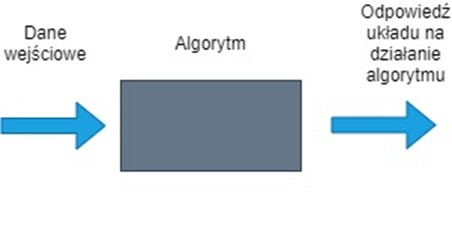
\includegraphics[scale=1.25]{image/Algorithms/Algorithm.jpg}
\caption{Uproszczony schemat blokowy każdego algorytmu}
\end{figure}

Każdy algorytm mozna przedstawić jako: 
\begin{itemize}
 \item Opis słowny
 \item Lista kroków
 \item Schemat blokowy
 \item Pseudokod
 
\end{itemize}

W kolejnych częściach pracy dyplomowej zostaną przedstawione metody prezentacji algorytmów na  przykładzie algorytmu NWD(Największy wspólny dzielnik)tzw. algorytm Euklidesa

\section{Opis słowny}

Opisanie procesu krótkimi zdaniami, które jednoznacznie sugerują wykonywaną czynność.
\newline
Wczytaj liczby a i b, które są liczbami naturalnymi. Dopóki liczby a i b są różne od siebie, odejmujemy 	liczbę mniejszą od większej. Gdy liczby a i b staną się sobie równe to NWD(a, b) jest dowolną liczbą, 	która została uzyskana w ostatnim kroku.

\section{Lista kroków}

Opisanie procesu za pomocą krótkich poleceń ponumerowanych w kolejności ich realizacji
\begin{enumerate}
	\item Wczytaj liczbę a zgodną z założeniami początkowymi algorytmu
	\item Wczytaj liczbę b zgodną z założeniami początkowymi algorytmu
	\item Jeżeli liczba b = 0 idź do kroku 6 w innym wypadku odejmij mniejszą liczbę 	od większej
	\item Większą liczbę zastąp mniejszą
	\item Mniejszą liczbę zastąp resztą z dzielenia (operacja modulo)
	\item Wróć do kroku 2
	\item Wypisz liczbę a
	\item Zakończ działanie programu
\end{enumerate}
\newpage
\section{Schemat blokowy}
Graficzna prezentacja kolejnych etapów, umożliwiających precyzyjne określenie 
wykonywanie czynności m.in. Rozpoczęcie algorytmu, zakończenie, wczytanie informacji, wyświetlenie informacji, lub bloku decyzyjnego.

\centering \begin{table} [ht]
 \caption{Przedstawienie podstawowych bloków używanych do tworzenia schematów blokowych}
 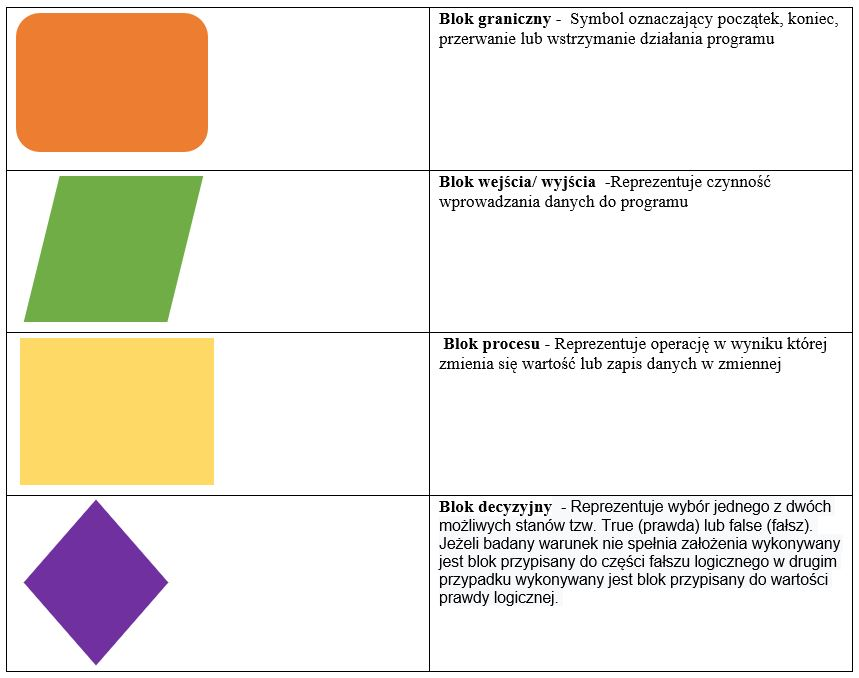
\includegraphics[scale=0.8]{image/table/table1.JPG}
\end{table}  

\begin{figure}[hp]
\centering
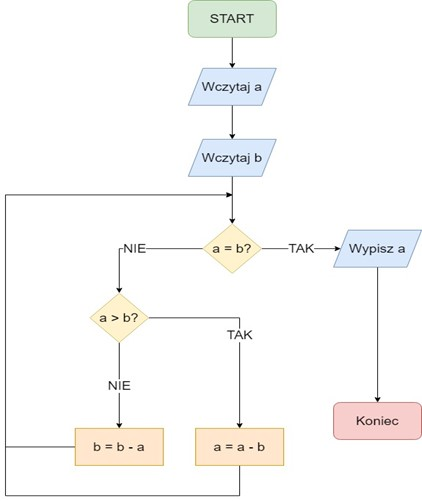
\includegraphics[scale = 1.4]{image/Algorithms/NWDalgorithm.jpg}
\caption{Schemat blokowy algorytmu Euklidesa}
\end{figure}

\newpage
\section{Pseudokod}
Prezentacja algorytmu podobnie jak w przypadku opisu słownego jednak w tym przypadku kolejne kroki zawierają kod przypominający składnię języka lub będący częścią składni m.in. średniki, dwukropki, wyrażenia typu for, while if itd.

\begin{figure}[h]
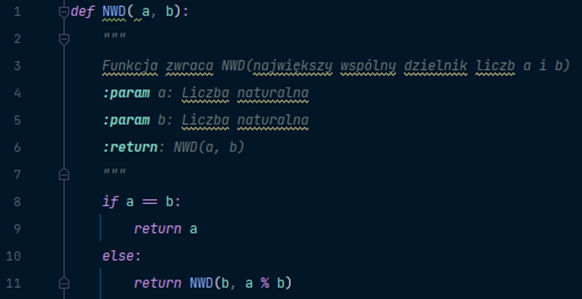
\includegraphics[scale=1.15]{image/code/code.png}
\caption{Program wykonujący algorytm Euklidesa w pseudokodzie języka Python}
\end{figure}


\chapter{Filtr cyfrowy}
Filtr cyfrowy jest programem komputerowym służącym do usunięcia niechcianych pasm częstotliwości lub innych składowych sygnałów.
Każdy z filtrów można projektować w dziedzinie czasu lub częstotliwości. Klasyczne filtry można projektować przy użyciu tzw. konwolucji( operacja splotu matematycznego) lub rekursji (rekurencji). Filtry można kategaryzować m.in ze względu  na charakterystyki na, których działa algorytm. 
\newline 
\begin{figure}[hp]
\centering
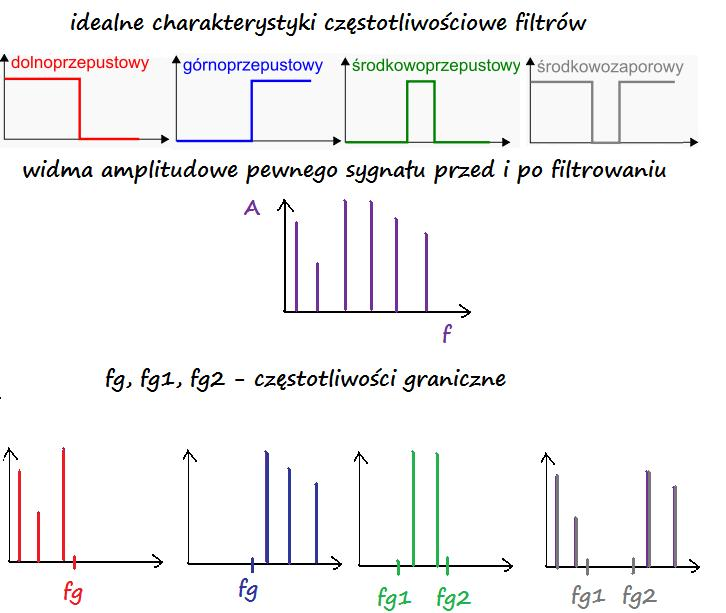
\includegraphics[scale=0.75]{image/rodzfiltrow.jpg}
\caption{Podział filtrów ze względu na charakterystyki pracy a) Dolnoprzepustowy, b) Górnoprzepustowy, c) Środkowoprzepustowy, d) Środkowozaporowy}
\end{figure}
\newpage
\begin{itemize}
\item Charakterystyka dolnoprzepustowa - Filtr "usuwa" częstotliwości powyżej zadanej częstotliwości, podobnie jak czerwona charakterystyka na rysunku 3.1
\item Charakterystyka górnoprzepustowa - Filtr "usuwa" częstotliwości poniżej zadanej częstotliwości, podobnie jak niebeiska charakterustyka na rysunku 3.1
\item Charakterystyka środkowoprzepustowa - Filtr "usuwa" częstotliwości poniżej oraz częstotliwości powyżej zadanego pasma, podobnie jak zielona charakterystyka na rysunku 3.1
\item Charakterystyka środkowozaporowa - Filtr "usuwa" częstotliwości w zadanym paśmie, tzn. działa w sposób odwrotny niż filtr środkowoprzepustowy, przykładem filtru jest szara charakterystyka  na rysunku 3.1
\end{itemize}

\begin{figure}[ht]
\centering
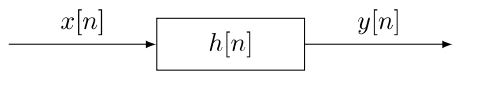
\includegraphics[scale=1.]{image/schemat_filtruJPG.JPG}
\caption{Ogólny schemat działania filtru cyfrowego, x(n) jest sygnałem wejściowym, h(n) rozumiemy jako operacje zachodzące wewnątrz filtru, natomiast y(n) jest sygnałem wyjściowym}
\end{figure}
%\section{Twierdzenie o próbkowaniu}
%Znane również jak Twierdzenie Kotielnikova-Shanona lub Twierdzenie Whittaker'a-Nyquist'a-%Kotielnikova-Shanona, którego treść brzmi następująco :  

%\begin{twr} [Twierdzenie Kotielnikowa-Shannona]
%Częstotliwośc próbkowania fs musi być nie mniejsza niż dwukrotność najwyższej składowej %częstotliwości badanego sygnału
%	\begin{equation}
%\label{eq:Twiedzenie_probkowania}
%	 f_{s} \geq 2  f_{p}
%\end{equation}
%\end{twr}

%Niepoprawne dobranie częstotliwości próbkowania $f_{p}$ (jest mniejsza niż dwukrotność %$f_{s}$) prowadzi do tzw. zjawiska aliasingu, którego skutkiem są błędy podczas operacji %translacji sygnału analogowego na sygnał cyfrowy.

%\section{Zjawisko Aliasingu}

\section{Filtr o skończonej odpowiedzi impulsowej (SOI)}

Filtry o skończonej odpowiedzi impulsowej będące tematem rozważań dla bieżącego podrozdziału do uzyskania aktualnej próbki sygnału wyjściowego korzystają ze zbioru przeszłych próbek wejściowych oraz próbki bieżącej. Filtr nie korzysta z próbek, które znajdują się na jego wyjściu dlatego również ten rodzaj filtru jest nazywany filtrem nierekursywnym. Do obliczenia wartości odpowiednich próbek wyjściowych filtr korzysta z operacji matematycznego dodawania w sposób podobny do procesu uśredniana.
 
\begin{figure}[h]
	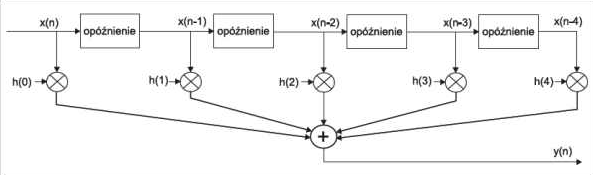
\includegraphics[scale=1.1]{image/fir.png}
	\caption{Schemat filtru cyfrowego typu SOI z rzędem filtru M = 5}
\end{figure}

\newpage
\begin{figure}[h]
	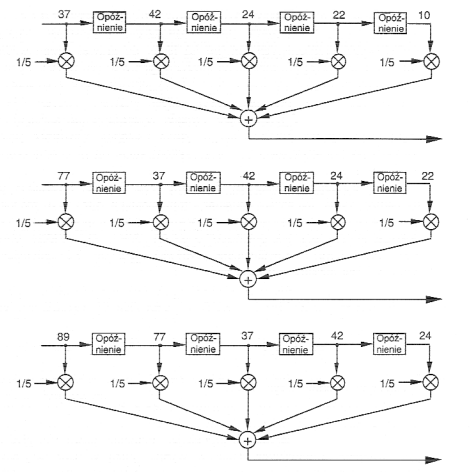
\includegraphics[scale=1.25]{image/firobliczenia.png}
	\caption{Przykładowe obliczenia wartości próbki dla filtru FIR rzędu M = 5}
\end{figure}

\begin{equation}
\label{eq:sumadluzsza}
	y_{wyj}(n) =  \frac{1}{5} x(k) = \frac{1}{5}x(n-4) + \frac{1}{5}x(n-3) +  \frac{1}{5}x(n-2) \frac{1}{5}x(n-1) + \frac{1}{5}x(n) 
\end{equation}

\newpage

\begin{equation}
\label{eq:sumakrotsza}	 
	 \sum_{k=n - 4}^{n} \frac{1}{5}x(k) 
\end{equation}

Zarówno równanie numer \ref{eq:sumadluzsza} jak również równanie \ref{eq:sumakrotsza} są tym samym równaniem w dłuższej i krótszej opcji zapisowej, pozwalającymi obliczyć n-tą próbkę w filtrze o rzędziu złożoności M.
\newline
Dla chwil a, b i c obliczono odpowiednio wartości piątej, szóstej oraz siódmej próbki wyjściowej:

a)$ y_{wyj}(5) = \frac{37 + 42 + 24 + 22 + 10}{5} = \frac{135}{5} = 27$
\newline
b)$ y_{wyj}(5) = \frac{77 + 37 + 42 + 24 + 22}{5} = \frac{202}{5} = 40,4$ 
\newline
c)$ y_{wyj}(5) = \frac{89 + 77 + 37 + 42 + 24}{5} = \frac{269}{5} = 53,8$
\newline


W rzeczywistości współczynniki filtrów posiadają różne wartości dlatego dla przykładów a,b,c oraz równań \ref{eq:sumadluzsza} i \ref{eq:sumakrotsza} odpowiednia będzie ogólna postać.
\begin{equation}
\label{eq:splocik}
 \sum_{k = 0}^M h(k) x(n-k)
\end{equation}

Równanie \ref{eq:splocik} jest równaniem splotu matematycznego. Jest to nic innego jak suma iloczynów jednak w tym przypadku przed przystąpieniem do obliczenia sum należy odwrócić kolejność czasową z jaką próbki wchodziły na wejście filtru FIR.


\chapter{Algorytm oparty na  strategiach ewolucyjnych lub hybrydowych}
\section{Algorytm Ewolucyjny}
Rodzina algorytmów, które do działania  podobnie jak sieci neuronowe wykorzystują techniki inspirowane analogiami biologicznymi. Algorytmy ewolucyjne zamiast wyszukiwać rozwiązania np.(metoda Brute force) starają się "wychodować" najlepsze możliwe rozwiązanie. Wychodowanie optymalnego rozwiązania wymaga szeregu operacji m.in. krzyżowania, rozmnażania, konkurencji itp. Algorytmy ewolucyjne (AE) wykorzystują nomenklaturę zaczerpniętę z genetyki :
\newline
\begin{itemize}
\item \textbf{Gen} - Najmniejsza jednostka algorytmu ewolucyjnego. Jest cechą, cząstką rozwiązania
\item \textbf{Osobnik} - Zbiór parametrów zadania będący potencjalnym rozwiązaniem problemu
\item \textbf{Chromosom} - Uporządkowany ciąg genów
\item \textbf{Locum} - Wskazuję miejsce położenia każdego z genów w chromosomie
\item \textbf{Genotyp} - Struktura złożona z chromosomów określonego osobnika 
\item \textbf{Fenotyp} - Zestaw wartości odpowiadających danemu genotypowi, będący jakością konkretnego osobnika
\item \textbf{Allel} - Określa wartość cechy konkretnego genu
\item \textbf{Populacja} - Zbiór osobników spełniające odpowiednie wartości danej cechy oraz spełniająca zdefiniowaną ilość osobników 
\end{itemize}


Każdy z algorytmów ewolucyjnych posiada szereg operacji charakterystycznych dla całej rodziny algorytmów czerpiących z teorii ewolucji:
\newline
\begin{enumerate}
\item Wytworzenie populacji złożonej ze zdefiniowanej ilości osobników, o wartościach spełniającymi ściśle zdefinowane wartości.
\begin{equation}
x_{n} \in \mathbb{Z}
\end{equation}
$x_{n}$ - Liczba osobników
\item Każdy osobnik będący w zbiorze populacji powinien zostać zaklasyfikowany przez specjalną funkcję klasyfikującą (fitness function), zdefiniowaną na etapie projektowania algorytmu. Wartość nadawana przez \textbf{fitness function} określa na ile rozwiązanie odbiega od rozwiązania optymalnego. Z tego wynika, że wartość idealnego rozwiązania powinna być bliska lub równa 0 \newline
\begin{equation}
\lim_{x_{n} \rightarrow 0} fitness(x_{n}) = 0 
\end{equation}
\item Kolejnym krokiem jest został spełnieny warunek dotyczący maksymalnej ilości cykli(iteracji) lub przystosowania najlepszego osobnika w obrębie całego dostępnego zbioru populacji
\item Selekcja osobników na podstawie ocen jakie zostały do nich przypisany przez funkcję przystosowania. Jedną z najpopularniejszych metod wykorzystywanych do selekcji jest tzw. metoda koła ruletki. Polega 
\item Wybrane osobniki podlegają operatorom genetycznym (korzyżowanie oraz mutacja)
\item Wytworzenie nowej populacji osobników będące skutkiem wykonania operacji genetycznych
\item Powrót do punktu numer 2
\end{enumerate}

Metody selekcji osobników:
\begin{itemize}
\item \textbf{Metoda koła ruletki} - Każdemu z osobników zostaje przydzielony wycinek koła odpowiadający wartości funckji przystosowania badanego osobnika. 
\item \textbf{Metoda turniejowa} - Osobniki zostają podzielone na podgupy, nastepnie każda z podgrup dokonuje selekcji najlepszego osobnika z punktu widzenia funkcji przystosowania 
\item \textbf{Strategia elitarna} - Osobniki o najlepszej wartości funkcji przystosowania z punktu widzenia algorytmu jest 'chroniony'. Zapobiega się aby osobnik o najlepsze wartości został utracony 
\item \textbf{Selekcja rankingowa} - Każdemu z osobników będących w zbiorze  populacji zostaje przypisana ranga skorelowana z wartością funkcji przystosowania dla konkretnego osobnika
\end{itemize}

\begin{figure}[h]
\centering
\label{fig:ra}
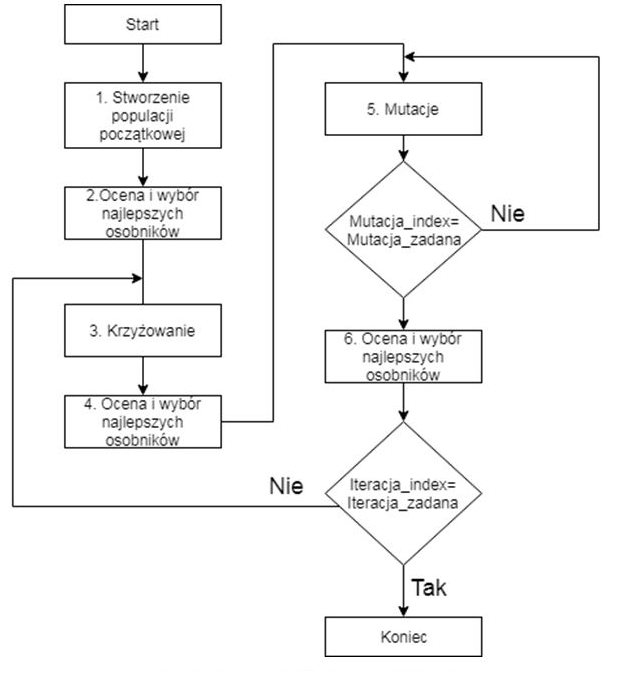
\includegraphics[scale=0.8]{image/Algorithms/ae.png}
\caption{Ogólny schemat blokowy algorytmu ewolucyjnego}
\end{figure}

\newpage
\subsection{Algorytm PSO}
Algorytm Particle Swarm Optimization został opublikowany w roku 1995 przez Panów James'a Kennedy'iego oraz Russel'a Eberhart'a. Metoda optymalizacji bazuje na dwóch innych metodach
\begin{itemize}
\item \textbf{Ewolucja obliczeniowa} - zastosowanie strategii ewolucyjnych, algorytmów genetycznych
\item Tzw. \textbf{Sztuczne życie} teoria roju, stada ptaków (powrót do miejsc, których w poprzednich okresach czasu(pobytu) lokalizowano pożywienie)
\end{itemize}

Zauważono, że stada lub ławice zwierząt wracają do miejść, w których odkryto pożywienie, w miejsca te docierały również osobniki, których wcześniej z racji na ich wiek nie było możliwe przemieszczenie. Dlatego obserwując skupienie osobników sformułowano cechy takie jak:
\begin{itemize}
\item \textbf{Bezpieczeństwo ruchu} - Zdolność do zapobiegania kolizji z obiektami będącymi przeszkodami lub osobnikami wewnątrz stada 
\item \textbf{Rozprzestrzenianie się} - Zdolność do rozproszenia stada, celem zarządzania odległościami pomiędzy osobnikami
\item \textbf{Orientacja} - Mozliwość znajdowania ustalonych miejsc, regionów punktów w przestrzeni poszukiwań 
\item \textbf{Skupianie} - Umiejętność gromadzenia się stada celem ustalenia maksymalnych odległości pomiędzy poszczególnymi osobnikami
\end{itemize}
Z punktu widzenia algorytmu PSO takie cechy jak rozprzestrzenianie się oraz bezpieczeństwo ruchu nie mają większego sensu dlatego zostały one wyeliminowane, okazało się, że zachowanie algorytmu koreluje w bliższy sposób z rojem aniżeli stadem/ławicą. Na podstawie własnych obserwacji oraz pracy Pana Milonas's zdefiniowano cechy roju takie jak: 
\begin{itemize}
\item \textbf{Jakość} - Jakość osobników jest zależna od zdefiniowanej funkcji klasyfikacyjnej
\item \textbf{Stabilność} - Populacja powinna być odporna na pewne bodźce (nie zmieniać zachowania mało znaczącej zmianie środowiska)
\item \textbf{Adaptacyjność} - Rój powinien ocenić czy zmiana zachowania jest opłacalna
\item \textbf{Różnorodność} - Rój powinien posiadać szeroki zbiór zachowań
\item \textbf{Bliskość} - Rój powinien być przechowywany w strukturze danych, która nie wymaga dużych nakładów złożoności obliczeniowej
\end{itemize}

Każdy z osobników powinien mieć informacje na temat:
\begin{itemize}
\item Własnej prędkości
\item Wartości funkcji klasyfikacyjnej dla obecnego oraz najlepszego swojego położenia
\item Swoje położenie w przestrzeni poszukiwań
\item Zbiór sąsiadów, położenie oraz wartość funkcji klasyfikacyjnej dla teego położenia
\end{itemize}


\newpage
\subsection{Schemat blokowy oraz parametry kontrolne}
\begin{figure}[ht]
\centering
\label{fig:cspso}
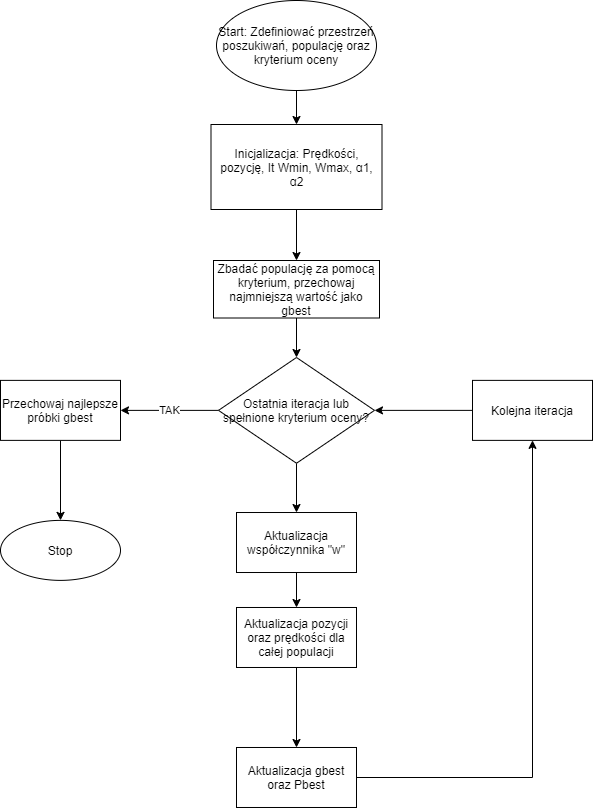
\includegraphics[scale=0.52]{image/schematy/PSO.png}
\caption{Schemat blokowy algorytmu PSO(Particle Swarm Optimization)}
\end{figure}

\begin{table}[bt]
\caption{Parametry kontrolne algorytmu PSO} % title of Table
\label{table:4_1}
\centering % used for centering table
\begin{tabular}{c c c c c} % centered columns (4 columns)
\hline\hline %inserts double horizontal lines
Parametry & PSO \\ [0.5ex] % inserts table
%heading
\hline % inserts single horizontal line
Wielkość populacji & 150 \\ % inserting body of the table
Ilość iteracji & 400 \\
$\alpha_{1}$, $\alpha_{2}$ & 1.9, 1.8 \\
$u_{min}$, $u_{max}$ & 0.01, 1.0 \\
$w_{min}$, $w_{max}$ & 0.4, 0.9 \\ [1ex] % [1ex] adds vertical space
Wartości brzegowe współczynników & [-1, 1] \\
\hline %inserts single line
\end{tabular}
\label{table:nonlin} % is used to refer this table in the text
\end{table}

\section{Algorytm hybrydowy}
\subsection{Algorytm CSPSO}
\newpage
\subsection{Schemat blokowy oraz parametry kontrolne}
\begin{figure}[!h]
\centering
\label{fig:cspso}
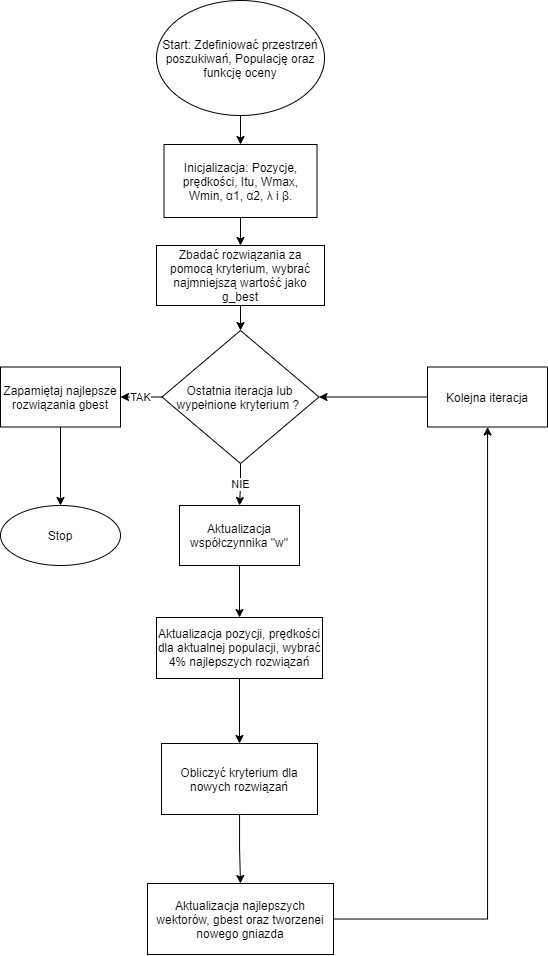
\includegraphics[scale=0.52]{image/schematy/CSPSO.png}
\caption{Schemat blokowy algorytmu CSPSO(Cuckoo Search Particle Swarm Optimization)}
\end{figure}

\begin{table}[ht]
\caption{Parametry kontrolne algorytmu CSPSO} % title of Table
\label{table:4_1}
\centering % used for centering table
\begin{tabular}{c c c c c} % centered columns (4 columns)
\hline\hline %inserts double horizontal lines
Parametry & CSPSO\\ [0.5ex] % inserts table
%heading
\hline % inserts single horizontal line
Wielkość populacji & 150\\ % inserting body of the table
Ilość iteracji & 400\\
$\alpha_{1}$, $\alpha_{2}$ & 1.9, 1.8\\
$u_{min}$, $u_{max}$ & 0.01, 1.0\\
$w_{min}$, $w_{max}$ & 0.4, 0.9\\ [1ex] % [1ex] adds vertical space

$\lambda$, $\beta$ & 1.1, 1.8 \\
Wartości brzegowe współczynników & [-1, 1]\\
\hline %inserts single line
\end{tabular}
\label{table:nonlin} % is used to refer this table in the text
\end{table}
\subsection{Funkcja Gamma ($\Gamma$)}

\begin{equation}
	\Gamma(z) = \int_{0}^{\infty} t^{z - 1}e^{-t}dt
	\label{eq:gamma}
\end{equation}
\subsection{Funckja lotu Levy'ego}
\begin{equation}
	s = \frac{u}{\vert v\vert^{1 / \beta}} 
\end{equation}

\begin{equation}
 u \sim N(0, \sigma^{2}_{n})
\end{equation}

\begin{equation}
 s \sim N(0, \sigma^{2}_{n})
\end{equation}

\begin{equation}
	\sigma_{u} =\lbrace \frac{\Gamma(1 + \beta) \sin{(\pi \beta / 2)}}{\Gamma\lbrack(1 + \beta) /2\rbrack \beta 2 ^{(\beta - 1) / 2}}\rbrace^{1 / \beta}
\end{equation}
\chapter{Implementacja}
\section{Algorytm PSO}
\subsection{Generowanie pojedynczego rozwiazania}
\begin{lstlisting}[language=Python, caption=Implementacja stworzenia pojedynczego rozwiązania]

def generate_solution(filter_order: int):
    solution = []
    for gene in range(0, filter_order):
        solution.append(random.uniform(-1, 1))
    return solution
\end{lstlisting}
\subsection{Generowanie prędkości}
\begin{lstlisting}[language=Python, caption=Generowanie prędkości]

def generate_velocities(v_min, v_max, order: int):
    velocities = []
    for i in range(0, order):
        velocities.append(random.uniform(v_min, v_max))
    return velocities
\end{lstlisting}

\subsection{Obliczenie $ V(\omega_{n})$}
\begin{lstlisting}[language=Python, caption=Implementacja równania Obliczenie $ V(\omega_{n})$]


def v_omega_n(order: int, solution):
    final = 0
    for m in range(0, order):
        omega = ((2 * np.pi * m) / (order + 1))
        final += solution[m] * np.exp(-1j * m * omega)
    return final
\end{lstlisting}
\subsection{Generowanie prędkości początkowych}
\begin{lstlisting}[language=Python, caption=Implementacja funkcji generuącej prędkośi dla każdej cząsteczki]

def generate_velocities(v_min, v_max, order: int):
    velocities = []
    for i in range(0, order):
        velocities.append(random.uniform(v_min, v_max))
    return velocities
\end{lstlisting}
\subsection{Obliczenie funkcji dopasowania}
\begin{lstlisting}[language=Python, caption=Implementacja funkcji klasyfikującej rozwiązanie]

def fitness_function(filter_order: int, v_a_omega, band_pass, band_stop):
    fitness = 0
    first_sume = 0
    second_sume = 0
    for gene in range(0, filter_order):
        first_sume += (np.abs(np.abs(v_a_omega) - 1) - band_pass) ** 2
        second_sume += (np.abs(v_a_omega) - band_stop) ** 2
        fitness += first_sume + second_sume
    return fitness
\end{lstlisting}
\subsection{Tworzenie nowych rozwiązań z obecnego pokolenia}
\begin{itemize}
\item Aktualizacja współczynnika $\omega$
\begin{lstlisting}[language=Python, caption=Implementacja aktualizacji współczynnika $\omega$]

def w_current(w_maximum, w_minimum, current_iteration: int, number_of_iterations: int):
    return w_maximum - (current_iteration - number_of_iterations) * (w_maximum - w_minimum)
\end{lstlisting}
\item Aktualizacja prędkości $U^{k + 1}_{i}$
\begin{lstlisting}[language=Python, caption=Implementacja aktualizacji współczynnika prędkości $U^{k + 1}_{i}$]

def u_ik_plus_one(w_k:float,u_k,alpha1,alpha2,r1,r2,p_best, p_current, g_best,size:int,order:int):
    u_k_plus_one = [[0] * order] * size
    for i in range(0, size):
        for j in range(0, order):
            u_k_plus_one[i][j]= w_k*u_k[i][j]+alpha1*r1* (p_best[j]-p_current[i][j])+alpha2*r2*(
                      g_best[j]-p_current[i][j])
    return u_k_plus_one
\end{lstlisting}
\item Aktualizacja populacji $P^{k + 1}_{i}$
\begin{lstlisting}[language=Python, caption=Implementacja aktualizacji współczynnika prędkości $P^{k + 1}_{i}$]
def pi_k_plus_one(p_current,u_k_plus_one,size,order):
    p_current_plus_one = [[0]*order]*size
    for i in range(0,size):
        for j in range(0,order):
            p_current_plus_one[i][j] = p_current[i][j] + u_k_plus_one[i][j]
    return p_current_plus_one
\end{lstlisting}

\end{itemize}

\subsection{Skrypt}

\begin{small}
\begin{lstlisting}[language=Python, caption=Implementacja skryptu z algorytmem PSO]

import numpy as np
import random

if __name__ == "__main__":
 order = 41
 size = 150
 search_space = int(order / (2 + 1))
 cycles = 400
 alpha = 0.5
 alpha_one = 1.9
 alpha_two = 1.8
 band_pass = 0.6
 band_stop = 0.2
 u_min = 0.01
 u_max = 1.00
 w_min = 0.4
 w_max = 0.9
 _lambda = 1.1
 beta = 1.8
 velocity_vec = []
 population = []
 fitness = []

 for i in range(0, size):
 solution = generate_solution(order)
 solution_omega = v_omega_n(order, solution)
 fitness_res = fitness_function(order,solution_omega, band_pass band_stop)
 population.append(solution)
 fitness.append(fitness_res)
 velocity_vec.append(generate_velocities(u_min,u_max, order))
 print(f"Fitness{i} is {fitness_res}")
 g_best_fitt = min(fitness)
 g_best = population[fitness.index(min(fitness))]
 p_best = g_best
  for iteration in range(0,cycles):
   local_fitness = 0
   r1 = r_generator()
   r2 = r_generator()
   w_k = w_current(w_max,w_min,iteration,cycles)
   u_ki=u_ik_plus_one(w_k,velocity_vec,alpha_one,/
   alpha_two,r1,r2,p_best,population,g_best,size,order)
   new_pop = pi_k_plus_one(population,u_ki,size,order)
    for solution in range(0,size):
     local_omega = v_omega_n(order,new_pop[solution])
     fitness = fitness_function(order,local_omega, band_pass,band_stop)
     p_best_fitenss = np.min(fitness)
     p_best = new_pop[fitness.index(p_best_fitenss)]
     if p_best_fitenss < g_best_fitt:
      g_best_fitt = p_best_fitenss
    print(g_best) 
\end{lstlisting}
\end{small}
\newpage
\section{Algorytm CSPSO}

\subsection{Generowanie pojedynczego rozwiazania}
\begin{lstlisting}[language=Python, caption=Implementacja stworzenia pojedynczego rozwiązania]

def generate_solution(filter_order: int):
    solution = []
    for gene in range(0, filter_order):
        solution.append(random.uniform(-1, 1))
    return solution
\end{lstlisting}
\subsection{Obliczenie $ V(\omega_{n})$}
\begin{lstlisting}[language=Python, caption=Implementacja równania Obliczenie $ V(\omega_{n})$]


def v_omega_n(order: int, solution):
    final = 0
    for m in range(0, order):
        omega = ((2 * np.pi * m) / (order + 1))
        final += solution[m] * np.exp(-1j * m * omega)
    return final
\end{lstlisting}
\subsection{Generowanie prędkości początkowych}
\begin{lstlisting}[language=Python, caption=Implementacja funkcji generuącej prędkośi dla każdej cząsteczki]

def generate_velocities(v_min, v_max, order: int):
    velocities = []
    for i in range(0, order):
        velocities.append(random.uniform(v_min, v_max))
    return velocities
\end{lstlisting}
\subsection{Obliczenie funkcji dopasowania}
\begin{lstlisting}[language=Python, caption=Implementacja funkcji klasyfikującej rozwiązanie]

def fitness_function(filter_order: int, v_a_omega, band_pass, band_stop):
    fitness = 0
    first_sume = 0
    second_sume = 0
    for gene in range(0, filter_order):
        first_sume += (np.abs(np.abs(v_a_omega) - 1) - band_pass) ** 2
        second_sume += (np.abs(v_a_omega) - band_stop) ** 2
        fitness += first_sume + second_sume
    return fitness
\end{lstlisting}
\subsection{Tworzenie nowych rozwiązań z obecnego pokolenia}
\begin{itemize}
\item Aktualizacja współczynnika $\omega$
\begin{lstlisting}[language=Python, caption=Implementacja aktualizacji współczynnika $\omega$]

def w_current(w_maximum, w_minimum, current_iteration: int, number_of_iterations: int):
    return w_maximum - (current_iteration - number_of_iterations) * (w_maximum - w_minimum)
\end{lstlisting}
\item Aktualizacja prędkości $U^{k + 1}_{i}$
\begin{lstlisting}[language=Python, caption=Implementacja aktualizacji współczynnika prędkości $U^{k + 1}_{i}$]

def u_ik_plus_one(w_k:float,u_k,alpha1,alpha2,r1,r2,p_best, p_current, g_best,size:int,order:int):
    u_k_plus_one = [[0] * order] * size
    for i in range(0, size):
        for j in range(0, order):
            u_k_plus_one[i][j]= w_k*u_k[i][j]+alpha1*r1* (p_best[j]-p_current[i][j])+alpha2*r2*(
                      g_best[j]-p_current[i][j])
    return u_k_plus_one
\end{lstlisting}
\item Aktualizacja populacji $P^{k + 1}_{i}$
\begin{lstlisting}[language=Python, caption=Implementacja aktualizacji współczynnika prędkości $P^{k + 1}_{i}$]
def pi_k_plus_one(p_current,u_k_plus_one,size,order):
    p_current_plus_one = [[0]*order]*size
    for i in range(0,size):
        for j in range(0,order):
            p_current_plus_one[i][j] = p_current[i][j] + u_k_plus_one[i][j]
    return p_current_plus_one
\end{lstlisting}

\end{itemize}
\newpage
\subsection{Funkcja Lotu Levy'ego}

\begin{lstlisting}[language=Python, caption=Implementacja funkcji Levy'ego, label={lst:6}]

   function nest=get_cuckoos(nest,best,Lb,Ub)
% Levy flights
n=size(nest,1);
% Levy exponent and coefficient
% For details, see equation (2.21), Page 16 (chapter 2) of the book
% X. S. Yang, Nature-Inspired Metaheuristic Algorithms, 2nd Edition, Luniver Press, (2010).
beta=3/2;
sigma=(gamma(1+beta)*sin(pi*beta/2)/(gamma((1+beta)/2)*beta*2^((beta-1)/2)))^(1/beta);
for j=1:n,
    s=squeeze(nest(j,:,:));


    % This is a simple way of implementing Levy flights
    % For standard random walks, use step=1;
    %% Levy flights by Mantegnas algorithm
    u=randn(size(s))*sigma;
    v=randn(size(s));
    step=u./abs(v).^(1/beta);


    % In the next equation, the difference factor (s-best) means that
    % when the solution is the best solution, it remains unchanged.
    stepsize=0.01*step.*(s-best);
    % Here the factor 0.01 comes from the fact that L/100 should the typical
    % step size of walks/flights where L is the typical lenghtscale;
    % otherwise, Levy flights may become too aggresive/efficient,
    % which makes new solutions (even) jump out side of the design domain
    % (and thus wasting evaluations).
    % Now the actual random walks or flights
    s=s+stepsize.*randn(size(s));
   % Apply simple bounds/limits
   %nest(j,:,:)=simplebounds(s,Lb,Ub);
end
        
\end{lstlisting}

\newpage

\begin{equation}
	w^k = w_{max} - \frac{k}{It_{u}}(w_{max} - w_{min})
	\label{eq:wk}
\end{equation}
\ref{eq:wk} Aktualizacja współczynnika $w^{k}$

\begin{lstlisting}
def w_current(w_maximum, w_minimum, current_iteration: int, number_of_iterations: int):
    return w_maximum - (current_iteration - number_of_iterations) * (w_maximum - w_minimum)
    \label{lst:wk}
\end{lstlisting}

\begin{equation}
	U^{(k + 1)}_{i} = w^{k}U^k_{i} + \alpha_{1}r_{1}(P_{best_{i}}^{k} - P^{k}_{i}) + \alpha_{2}r_{2} (g^{k}_{best} - P^k_{i})
	\label{eq:uk1}
\end{equation}
\ref{uk1} Obliczenie prędkości dla kolejnego pokolenia rozwiązań

\begin{lstlisting}
def u_ik_plus_one(w_k, u_k, alpha1, alpha2, r1, r2, pbest, pcurrent, g_best_current):
    return w_k * u_k + alpha1 * r1(pbest - pcurrent) + alpha2 * r2 * (g_best_current - pcurrent)
\end{lstlisting}
\begin{equation}
	P^{(k + 1)}_{i} = P^{k}_{i} + U^{(k + 1)}_{i}
	\label{eq:pk1}
\end{equation}
\ref{eq:pk1} Obliczenie pozycji dla kolejnego pokolenia rozwiązań

\begin{lstlisting}
def pi_k_plus_one(p_current, u_k_plus_one):

    return p_current + u_k_plus_one
\end{lstlisting}

\chapter{Podsumowanie}
\chapter*{Literatura}
\begin{thebibliography}{3}
\bibtem{bib_element1}
\end{thebibliography}

\listoftables

\listoffigures

\end{document}
